\documentclass[11pt,a4paper]{article}
\usepackage{amsmath}\usepackage{amssymb}\usepackage[table]{xcolor}
\usepackage{tabularx}\usepackage{multirow}\usepackage{geometry}
\usepackage{enumitem}\usepackage{parskip}\usepackage{titlesec}
\usepackage{tocloft}\usepackage[most]{tcolorbox}
\usepackage{tikz}\usepackage{pgfplots}\pgfplotsset{compat=1.18}\usetikzlibrary{arrows.meta,calc,positioning,shapes.geometric,patterns}
\geometry{margin=2.5cm}
\titleformat{\section}{\large\bfseries}{}{0em}{}
\setlength{\cftbeforesecskip}{6pt}
\definecolor{q1color}{HTML}{D6EAF8}\definecolor{q2color}{HTML}{D5F5E3}
\definecolor{q3color}{HTML}{FDEBD0}\definecolor{q4color}{HTML}{F9E79F}
\definecolor{q5color}{HTML}{E8DAEF}\definecolor{q6color}{HTML}{FADBD8}
\definecolor{q7color}{HTML}{D1F2EB}\definecolor{q8color}{HTML}{FCF3CF}
\definecolor{q9color}{HTML}{EBDEF0}\definecolor{q10color}{HTML}{F5EEF8}
\newenvironment{mstab}[1]{%
  {\color{#1!75!black}\nobreak Mark Scheme}\par\nopagebreak\smallskip
  \arrayrulecolor{#1!70!black}\renewcommand{\arraystretch}{1.3}%
  \tabularx{\textwidth}{|>{\columncolor{#1!12}\raggedright\arraybackslash}p{1.9cm}|>{\columncolor{#1!12}}X|>{\columncolor{#1!12}\centering\arraybackslash}p{1.1cm}|}%
  \hline\rowcolor{#1!45} Question & Answer & Marks \\ \hline}{%
  \endtabularx\arrayrulecolor{black}\par\medskip}
\newtcolorbox{ansbox}[1]{colback=#1!8,colbacktitle=#1!30,colframe=#1!70!black,coltitle=black,fonttitle=\normalfont,title=Worked Solution,boxrule=0.6pt,arc=2mm,left=4pt,right=4pt,top=4pt,bottom=4pt,breakable}
\newcommand{\topiclabel}[1]{\hfill\normalfont\small\itshape\textcolor{black!55}{#1}}
\newcommand{\examq}[4]{\section[#1 - Q#2]{#1 - Q#2 - #3 - #4}}
\begin{document}
\begin{center}
  {\LARGE \textbf{Cambridge O Level Mathematics (Syllabus D) 4024/11/O/N/24}}\\[6pt]
  {\large October/November 2024 -- Mark Scheme \& Worked Solutions}
\end{center}
\bigskip

%========================= Q1 =========================
\examq{4024/11/O/N/24}{1}{Number Fundamentals}{2}

\begin{mstab}{q1color}
1(a) & 6 & 1 \\ \hline
1(b) & $-11$ & 1 \\ \hline
\end{mstab}

\begin{ansbox}{q1color}
\textbf{(a)} The difference is the higher temperature minus the lower one.
\[ 4 - (-2) = 4 + 2 = 6 \]
The difference is $6\,^{\circ}\mathrm{C}$.

\textbf{(b)} ``$9$ degrees lower'' means subtract $9$ from the midday temperature.
\[ -2 - 9 = -11 \]
The temperature at midnight is $-11\,^{\circ}\mathrm{C}$.
\end{ansbox}

%========================= Q2 =========================
\examq{4024/11/O/N/24}{2}{Ratio \& Proportion}{2}

\begin{mstab}{q2color}
2 & 200 \newline M1 for $\dfrac{280}{7} \times k$ oe where $k = 1$, 2 or 5 & 2 \\ \hline
\end{mstab}

\begin{ansbox}{q2color}
The ratio $2 : 5$ splits the money into $2 + 5 = 7$ equal parts.
\[ 1 \text{ part} = \frac{280}{7} = 40 \]
Pablo has $5$ parts.
\[ 5 \times 40 = 200 \]
Pablo's share is $\$200$. (Check: Amber gets $2 \times 40 = \$80$, and $80 + 200 = 280$.)
\end{ansbox}

%========================= Q3 =========================
\examq{4024/11/O/N/24}{3}{Averages \& Range}{3}

\begin{mstab}{q3color}
3(a) & $-1$ & 1 \\ \hline
3(b) & $-2$ \newline B1 for $-7$ $-5$ $-3$ $-3$ $-1$ $-1$ $-1$ 2 soi & 2 \\ \hline
\end{mstab}

\begin{ansbox}{q3color}
\textbf{(a)} The mode is the value appearing most often. In the list $-1$, $-5$, $-1$, $-3$, $-3$, $2$, $-1$, $-7$ the value $-1$ appears three times, more than any other.
\[ \text{mode} = -1 \]

\textbf{(b)} Put the eight integers in order first, remembering that the more negative a number is, the smaller it is.
\[ -7,\ -5,\ -3,\ -3,\ -1,\ -1,\ -1,\ 2 \]
With eight values the median is the mean of the $4$th and $5$th.
\[ \frac{-3 + (-1)}{2} = \frac{-4}{2} = -2 \]
\end{ansbox}

%========================= Q4 =========================
\examq{4024/11/O/N/24}{4}{Geometric Fundamentals}{2}

\begin{mstab}{q4color}
4(a) & & 1 \\ \hline
4(b) & 3 & 1 \\ \hline
\end{mstab}

\begin{ansbox}{q4color}
\textbf{(a)} A shape has a line of symmetry when folding along that line matches the two halves exactly. Look for a nearly-symmetrical arrangement in the given shading: there will be one square whose mirror image across a horizontal, vertical or diagonal fold line is currently unshaded. Shade that one square, then check the fold by eye before moving on.

\textbf{(b)} A regular polygon with $n$ sides has rotational symmetry of order $n$, because turning it through $\dfrac{360^{\circ}}{n}$ each time brings it back onto itself.

The polygon shown is an equilateral triangle, so
\[ \text{order} = 3 \]
\end{ansbox}

%========================= Q5 =========================
\examq{4024/11/O/N/24}{5}{Algebra Fundamentals \textperiodcentered\ Expanding \& Factorising Brackets}{3}

\begin{mstab}{q5color}
5(a) & $-3a + b$ final answer \newline B1 for $-3a$ or $[+]b$ in final answer or for $-3a + b$ seen & 2 \\ \hline
5(b) & $15x - 10$ final answer & 1 \\ \hline
\end{mstab}

\begin{ansbox}{q5color}
\textbf{(a)} Collect the $a$ terms and the $b$ terms separately.
\[ 2a - 3b + 4b - 5a \]
\[ = (2a - 5a) + (-3b + 4b) \]
\[ = -3a + b \]

\textbf{(b)} Multiply everything inside the bracket by $5$.
\[ 5(3x - 2) = 5 \times 3x - 5 \times 2 = 15x - 10 \]
\end{ansbox}

%========================= Q6 =========================
\examq{4024/11/O/N/24}{6}{Scatter Graphs \& Correlation}{4}

\begin{mstab}{q6color}
6(a) & Four points plotted correctly \newline B1 for 2 or 3 correct plots & 2 \\ \hline
6(b) & Ruled line of best fit & 1 \\ \hline
6(c) & Reading their straight line of best fit at 6 errors \newline Dependent on negative gradient & 1 \\ \hline
\end{mstab}

\begin{ansbox}{q6color}
\textbf{(a)} Six points are already plotted, so the four still to add are the last four pairs in the table.
\[ (60, 9) \qquad (65, 7) \qquad (63, 8) \qquad (70, 7) \]

\textbf{(b)} Rule one straight line through the middle of the ten points. The points fall from top-left to bottom-right, so the line must have a \emph{negative} gradient: more time spent means fewer errors.

\textbf{(c)} Go across from $6$ on the errors axis to the line of best fit, then down to the time axis. On a reasonable line the reading is about
\[ 73 \text{ minutes} \]
Any value read correctly from the candidate's own line is accepted.

\begin{center}
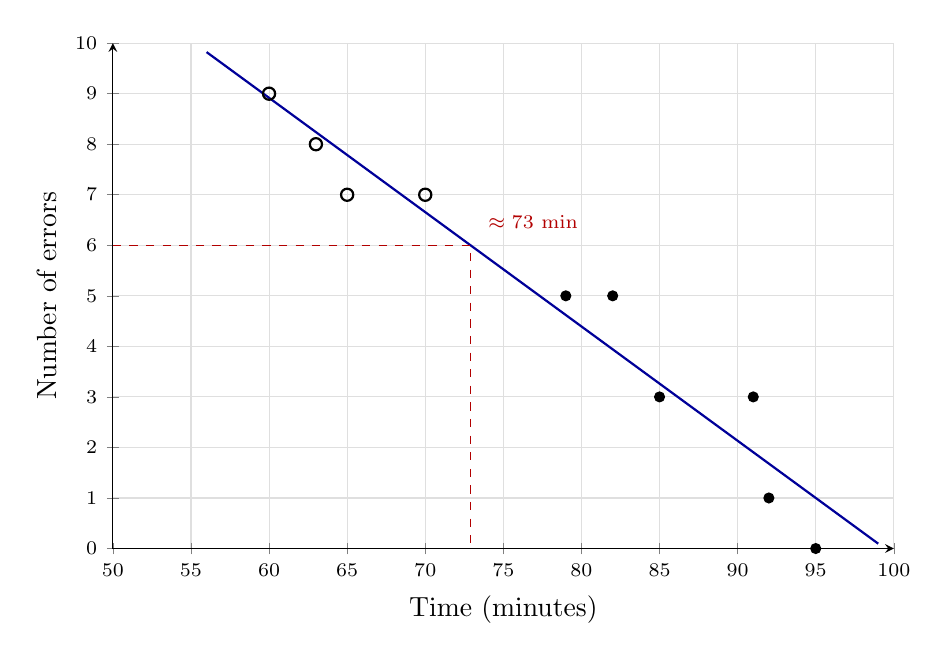
\begin{tikzpicture}
\begin{axis}[
  width=11.5cm, height=8cm,
  xmin=50, xmax=100, ymin=0, ymax=10,
  xtick={50,55,60,65,70,75,80,85,90,95,100},
  ytick={0,1,2,3,4,5,6,7,8,9,10},
  xlabel={Time (minutes)}, ylabel={Number of errors},
  grid=both, grid style={gray!25},
  tick label style={font=\scriptsize},
  axis lines=left]
  \addplot[only marks, mark=*, mark size=1.8pt]
    coordinates {(79,5) (92,1) (91,3) (85,3) (82,5) (95,0)};
  \addplot[only marks, mark=o, mark size=2.2pt, thick]
    coordinates {(60,9) (65,7) (63,8) (70,7)};
  \addplot[thick, blue!60!black, domain=56:99]{22.49 - 0.2262*x};
  \draw[dashed, red!70!black] (axis cs:50,6) -- (axis cs:72.9,6) -- (axis cs:72.9,0);
  \node[anchor=west, font=\scriptsize, red!70!black] at (axis cs:73.4,6.45) {$\approx 73$ min};
\end{axis}
\end{tikzpicture}
\end{center}
The four hollow points are the ones added in part (a).
\end{ansbox}

%========================= Q7 =========================
\examq{4024/11/O/N/24}{7}{Rounding, Estimation \& Bounds}{2}

\begin{mstab}{q7color}
7 & 3, 30, 7 and 2 seen as rounded values and final answer 18 \newline B1 for three of 3, 30, 7, 2 seen as rounded values & 2 \\ \hline
\end{mstab}

\begin{ansbox}{q7color}
Round each of the four numbers to $1$ significant figure.
\[ 3.1 \approx 3 \qquad 26.7 \approx 30 \qquad 6.9 \approx 7 \qquad 2.3 \approx 2 \]
Substitute the rounded values.
\[ \frac{3.1 \times 26.7}{6.9 - 2.3} \;\approx\; \frac{3 \times 30}{7 - 2} \]
\[ = \frac{90}{5} = 18 \]
The estimate is $18$.
\end{ansbox}

%========================= Q8 =========================
\examq{4024/11/O/N/24}{8}{Sequences}{3}

\begin{mstab}{q8color}
8(a) & 26 & 1 \\ \hline
8(b) & $6n - 4$ oe final answer \newline B1 for answer $6n + j$ or $kn - 4$, $k \neq 0$ \newline or for $6n - 4$ oe seen & 2 \\ \hline
\end{mstab}

\begin{ansbox}{q8color}
\textbf{(a)} The terms $2$, $8$, $14$, $20$ go up by $6$ each time.
\[ 20 + 6 = 26 \]

\textbf{(b)} A constant first difference of $6$ means the $n$th term starts with $6n$. Compare $6n$ with the sequence:
\[ 6n: \quad 6,\ 12,\ 18,\ 24 \]
\[ \text{sequence}: \quad 2,\ 8,\ 14,\ 20 \]
Each term is $4$ less than the matching multiple of $6$.
\[ n\text{th term} = 6n - 4 \]
Check with $n = 4$: $24 - 4 = 20$ \checkmark
\end{ansbox}

%========================= Q9 =========================
\examq{4024/11/O/N/24}{9}{Transformations}{5}

\begin{mstab}{q9color}
9(a) & Enlargement \newline [scale factor] 3 \newline [Centre] $(3, 4)$ \newline B1 for each & 3 \\ \hline
9(b) & Triangle drawn with vertices at $(-2, 5)$, $(-2, 3)$ and $(-1, 3)$ \newline B1 for triangle drawn after translation of $\begin{pmatrix} -3 \\ y \end{pmatrix}$ or triangle drawn after translation of $\begin{pmatrix} x \\ 2 \end{pmatrix}$ \newline If 0 scored, SC1 for translation of shape $B$ by $\begin{pmatrix} -3 \\ 2 \end{pmatrix}$ & 2 \\ \hline
\end{mstab}

\begin{ansbox}{q9color}
Triangle $A$ has vertices $(1, 3)$, $(1, 1)$ and $(2, 1)$, and triangle $B$ has vertices $(-3, 1)$, $(-3, -5)$ and $(0, -5)$.

\textbf{(a)} Triangle $B$ is three times as long in each direction as triangle $A$, so the transformation is an \textbf{enlargement} with \textbf{scale factor 3}.

To find the centre, join each vertex of $A$ to its image on $B$ and extend the lines back until they meet. Checking the candidate centre $(3, 4)$ with the rule
\[ \text{image} = (3, 4) + 3\big[\text{point} - (3, 4)\big] \]
\[ (1, 3) \mapsto (3, 4) + 3(-2, -1) = (-3, 1) \quad \checkmark \]
\[ (1, 1) \mapsto (3, 4) + 3(-2, -3) = (-3, -5) \quad \checkmark \]
\[ (2, 1) \mapsto (3, 4) + 3(-1, -3) = (0, -5) \quad \checkmark \]
So the description is: enlargement, scale factor $3$, \textbf{centre $(3, 4)$}. All three parts are needed.

\textbf{(b)} The translation $\begin{pmatrix} -3 \\ 2 \end{pmatrix}$ means $3$ to the left and $2$ up. Apply it to each vertex of $A$.
\[ (1, 3) \mapsto (-2, 5) \qquad (1, 1) \mapsto (-2, 3) \qquad (2, 1) \mapsto (-1, 3) \]

\begin{center}
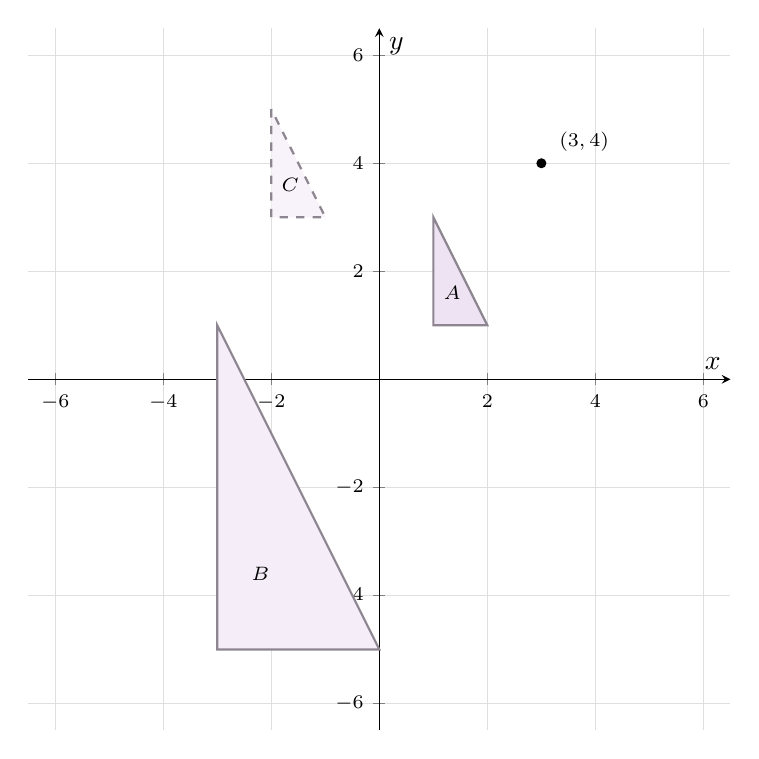
\begin{tikzpicture}
\begin{axis}[
  width=10.5cm, height=10.5cm,
  axis lines=middle,
  xmin=-6.5, xmax=6.5, ymin=-6.5, ymax=6.5,
  xtick={-6,-4,-2,2,4,6}, ytick={-6,-4,-2,2,4,6},
  xlabel={$x$}, ylabel={$y$},
  grid=both, grid style={gray!25},
  tick label style={font=\scriptsize},
  clip=true]
  \draw[fill=q9color!85, draw=q9color!60!black, thick]
    (axis cs:1,3) -- (axis cs:1,1) -- (axis cs:2,1) -- cycle;
  \draw[fill=q9color!50, draw=q9color!60!black, thick]
    (axis cs:-3,1) -- (axis cs:-3,-5) -- (axis cs:0,-5) -- cycle;
  \draw[fill=q9color!35, draw=q9color!60!black, thick, dashed]
    (axis cs:-2,5) -- (axis cs:-2,3) -- (axis cs:-1,3) -- cycle;
  \node[font=\scriptsize] at (axis cs:1.35,1.6) {$A$};
  \node[font=\scriptsize] at (axis cs:-2.2,-3.6) {$B$};
  \node[font=\scriptsize] at (axis cs:-1.65,3.6) {$C$};
  \addplot[only marks, mark=*, mark size=1.6pt] coordinates {(3,4)};
  \node[anchor=west, font=\scriptsize] at (axis cs:3.15,4.4) {$(3,4)$};
\end{axis}
\end{tikzpicture}
\end{center}
\end{ansbox}

%========================= Q10 =========================
\examq{4024/11/O/N/24}{10}{Simultaneous Equations}{3}

\begin{mstab}{q10color}
 & Correct method to eliminate one variable & M1 \\
\multirow{-2}{1.9cm}{10} & $a = -3$ \newline $b = 5$ \newline A1 for either $a = -3$ or $b = 5$ \newline If A0 scored, SC1 for a pair of values that satisfy either equation or for correct answers with no working & A2 \\ \hline
\end{mstab}

\begin{ansbox}{q10color}
\[ 3a + b = -4 \qquad \cdots (1) \]
\[ 2a + 3b = 9 \qquad \cdots (2) \]
Multiply equation $(1)$ by $3$ so that the $b$ terms match.
\[ 9a + 3b = -12 \qquad \cdots (3) \]
Subtract $(2)$ from $(3)$ to eliminate $b$.
\[ (9a - 2a) + (3b - 3b) = -12 - 9 \]
\[ 7a = -21 \]
\[ a = -3 \]
Substitute $a = -3$ into equation $(1)$.
\[ 3(-3) + b = -4 \]
\[ -9 + b = -4 \]
\[ b = 5 \]
Check in equation $(2)$: $2(-3) + 3(5) = -6 + 15 = 9$ \checkmark
\end{ansbox}

%========================= Q11 =========================
\examq{4024/11/O/N/24}{11}{Coordinate Geometry}{3}

\begin{mstab}{q1color}
11(a) & $(3.5$ oe$,\ 1)$ & 1 \\ \hline
11(b) & $-2$ \newline M1 for $\dfrac{-2 - 4}{5 - 2}$ oe & 2 \\ \hline
\end{mstab}

\begin{ansbox}{q1color}
\textbf{(a)} The midpoint is the mean of the two $x$-coordinates and the mean of the two $y$-coordinates, using $A(2, 4)$ and $B(5, -2)$.
\[ x = \frac{2 + 5}{2} = \frac{7}{2} = 3.5 \qquad y = \frac{4 + (-2)}{2} = \frac{2}{2} = 1 \]
The midpoint is $(3.5,\ 1)$.

\textbf{(b)} Gradient is the change in $y$ divided by the change in $x$.
\[ m = \frac{-2 - 4}{5 - 2} = \frac{-6}{3} = -2 \]
\end{ansbox}

%========================= Q12 =========================
\examq{4024/11/O/N/24}{12}{Powers, Roots \& Standard Form}{3}

\begin{mstab}{q2color}
12(a) & $2.57 \times 10^{-4}$ cao & 1 \\ \hline
12(b) & $5 \times 10^{8}$ cao \newline B1 for $0.5 \times 10^{9}$ oe seen \newline or for answer $A \times 10^{8}$ with $1 \leqslant A < 10$ & 2 \\ \hline
\end{mstab}

\begin{ansbox}{q2color}
\textbf{(a)} Standard form is $a \times 10^{n}$ with $1 \leqslant a < 10$. Moving the point in $0.000257$ four places right gives $2.57$, and moving right means a negative index.
\[ 0.000257 = 2.57 \times 10^{-4} \]

\textbf{(b)} Divide the numbers and the powers of ten separately.
\[ \frac{2 \times 10^{4}}{4 \times 10^{-5}} = \frac{2}{4} \times \frac{10^{4}}{10^{-5}} \]
\[ = 0.5 \times 10^{4 - (-5)} = 0.5 \times 10^{9} \]
This is not yet in standard form, since $0.5 < 1$. Write $0.5$ as $5 \times 10^{-1}$.
\[ 0.5 \times 10^{9} = 5 \times 10^{-1} \times 10^{9} = 5 \times 10^{8} \]
\end{ansbox}

%========================= Q13 =========================
\examq{4024/11/O/N/24}{13}{Fractions Fundamentals}{2}

\begin{mstab}{q3color}
13 & $2\dfrac{14}{15}$ cao \newline M1 for $\dfrac{11}{5} \times \dfrac{4}{3}$ or $\dfrac{44}{20} \div \dfrac{15}{20}$ oe & 2 \\ \hline
\end{mstab}

\begin{ansbox}{q3color}
Change the mixed number into an improper fraction.
\[ 2\tfrac{1}{5} = \frac{10 + 1}{5} = \frac{11}{5} \]
To divide by a fraction, multiply by its reciprocal.
\[ \frac{11}{5} \div \frac{3}{4} = \frac{11}{5} \times \frac{4}{3} \]
\[ = \frac{44}{15} \]
The question asks for a mixed number, so divide $44$ by $15$.
\[ 44 = 2 \times 15 + 14 \]
\[ \frac{44}{15} = 2\frac{14}{15} \]
Since $14$ and $15$ share no factor, this is already in its simplest form.
\end{ansbox}

%========================= Q14 =========================
\examq{4024/11/O/N/24}{14}{Prime Factors, HCF \& LCM}{3}

\begin{mstab}{q4color}
14(a) & $2^3 \times 3^2 \times 5$ or $2 \times 2 \times 2 \times 3 \times 3 \times 5$ \newline B1 for 2, 2, 2, 3, 3, 5 listed, not a product \newline or M1 for any two stages correct in factor tree or ladder method & 2 \\ \hline
14(b) & 75 & 1 \\ \hline
\end{mstab}

\begin{ansbox}{q4color}
\textbf{(a)} Divide by primes repeatedly.
\[ 360 = 2 \times 180 = 2 \times 2 \times 90 = 2 \times 2 \times 2 \times 45 = 2 \times 2 \times 2 \times 3 \times 15 \]
\[ = 2 \times 2 \times 2 \times 3 \times 3 \times 5 \]
\[ 360 = 2^3 \times 3^2 \times 5 \]

\textbf{(b)} A cube number has every prime index a multiple of $3$. Looking at $360n = 2^3 \times 3^2 \times 5 \times n$:
\begin{itemize}[nosep,leftmargin=*]
  \item the index of $2$ is already $3$, so no more $2$s are needed;
  \item the index of $3$ is $2$, so one more $3$ is needed to reach $3^3$;
  \item the index of $5$ is $1$, so two more $5$s are needed to reach $5^3$.
\end{itemize}
The smallest such $n$ is therefore
\[ n = 3 \times 5^2 = 3 \times 25 = 75 \]
Check: $360 \times 75 = 27\,000 = 30^3$ \checkmark
\end{ansbox}

%========================= Q15 =========================
\examq{4024/11/O/N/24}{15}{Circles, Arcs \& Sectors}{4}

\begin{mstab}{q5color}
15 & $24\pi$ nfww \newline B2 for $r = 12$ \newline or M1 for $\dfrac{60}{360} \times 2\pi r = 4\pi$ oe \newline AND \newline M1 for $\dfrac{60}{360} \times \pi \times (\text{their } r)^2$ oe & 4 \\ \hline
\end{mstab}

\begin{ansbox}{q5color}
The arc length of a sector is $\dfrac{\text{angle}}{360} \times 2\pi r$. Use the given arc length to find $r$ first.
\[ \frac{60}{360} \times 2\pi r = 4\pi \]
\[ \frac{1}{6} \times 2\pi r = 4\pi \]
\[ \frac{\pi r}{3} = 4\pi \]
Divide both sides by $\pi$, then multiply by $3$.
\[ r = 12 \]
Now use the sector area formula $\dfrac{\text{angle}}{360} \times \pi r^2$.
\[ \text{area} = \frac{60}{360} \times \pi \times 12^2 \]
\[ = \frac{1}{6} \times 144\pi = 24\pi \]
The area of the sector is $24\pi\ \mathrm{cm^2}$.
\end{ansbox}

%========================= Q16 =========================
\examq{4024/11/O/N/24}{16}{TOPIC NOT IN LIST -- matrices}{4}

\begin{mstab}{q6color}
16(a) & $\begin{pmatrix} -5 & 5 \\ 6 & 3 \end{pmatrix}$ \newline B1 for two or three correct elements \newline or for $\begin{pmatrix} -6 & 2 \\ 4 & 8 \end{pmatrix}$ seen & 2 \\ \hline
16(b)(i) & $-3$ & 1 \\ \hline
16(b)(ii) & $\dfrac{1}{10}\begin{pmatrix} 1 & -\text{their } k \\ -2 & 4 \end{pmatrix}$ oe \newline FT their $k$ & 1 \\ \hline
\end{mstab}

\begin{ansbox}{q6color}
\textbf{(a)} Multiply the first matrix by the scalar $2$, element by element, then subtract the second matrix element by element.
\[ 2\begin{pmatrix} -3 & 1 \\ 2 & 4 \end{pmatrix} = \begin{pmatrix} -6 & 2 \\ 4 & 8 \end{pmatrix} \]
\[ \begin{pmatrix} -6 & 2 \\ 4 & 8 \end{pmatrix} - \begin{pmatrix} -1 & -3 \\ -2 & 5 \end{pmatrix} = \begin{pmatrix} -6 - (-1) & 2 - (-3) \\ 4 - (-2) & 8 - 5 \end{pmatrix} \]
\[ = \begin{pmatrix} -5 & 5 \\ 6 & 3 \end{pmatrix} \]

\textbf{(b)(i)} For $\mathbf{A} = \begin{pmatrix} a & b \\ c & d \end{pmatrix}$ the determinant is $ad - bc$. Here $\mathbf{A} = \begin{pmatrix} 4 & k \\ 2 & 1 \end{pmatrix}$.
\[ 4 \times 1 - k \times 2 = 10 \]
\[ 4 - 2k = 10 \]
\[ -2k = 6 \]
\[ k = -3 \]

\textbf{(b)(ii)} The inverse is $\dfrac{1}{ad - bc}\begin{pmatrix} d & -b \\ -c & a \end{pmatrix}$, and the determinant is $10$.
\[ \mathbf{A}^{-1} = \frac{1}{10}\begin{pmatrix} 1 & -k \\ -2 & 4 \end{pmatrix} \]
With $k = -3$ this becomes
\[ \mathbf{A}^{-1} = \frac{1}{10}\begin{pmatrix} 1 & 3 \\ -2 & 4 \end{pmatrix} \]
\end{ansbox}

%========================= Q17 =========================
\examq{4024/11/O/N/24}{17}{Solving \& Graphing Inequalities}{4}

\begin{mstab}{q7color}
17(a) & B1 for $y = -2$ drawn \newline or for a region between the two boundary lines identified & 2 \\ \hline
17(b) & 0, 1, 2 \newline B1 for 2 correct with no errors \newline or 3 correct with one error \newline or for coordinates of a point on the line $y = x - 2$ identified & 2 \\ \hline
\end{mstab}

\begin{ansbox}{q7color}
\textbf{(a)} The two lines $y = 2x + 1$ and $x + y = 2$ are already drawn, so the only line still needed is $y = -2$, a horizontal line. Then keep the correct side of each boundary.
\begin{itemize}[nosep,leftmargin=*]
  \item $y \leqslant 2x + 1$: keep the side \emph{below} the steep line.
  \item $x + y \leqslant 2$: keep the side \emph{below} the falling line.
  \item $y \geqslant -2$: keep the side \emph{above} the horizontal line.
\end{itemize}
The three boundaries meet in pairs at $(-1.5, -2)$, $\left(\tfrac{1}{3}, \tfrac{5}{3}\right)$ and $(4, -2)$, so $R$ is the triangle with those vertices.

\begin{center}
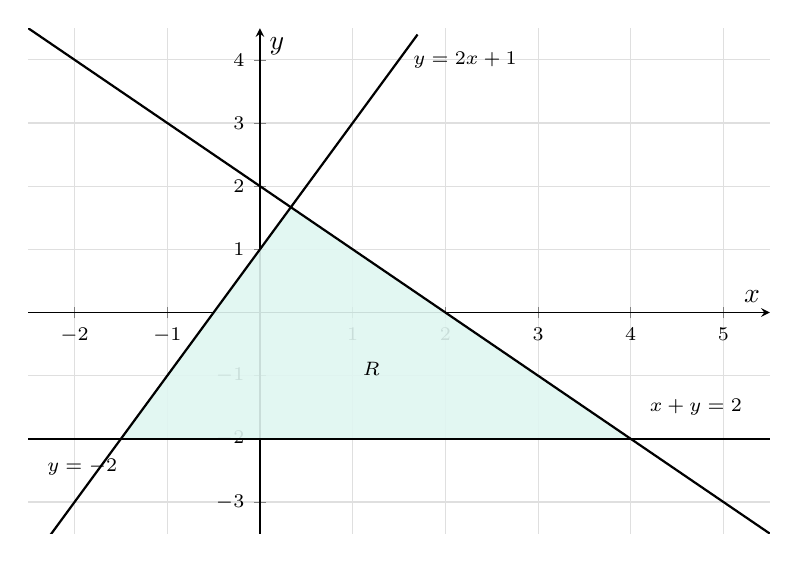
\begin{tikzpicture}
\begin{axis}[
  width=11cm, height=8cm,
  axis lines=middle,
  xmin=-2.5, xmax=5.5, ymin=-3.5, ymax=4.5,
  xtick={-2,-1,1,2,3,4,5}, ytick={-3,-2,-1,1,2,3,4},
  xlabel={$x$}, ylabel={$y$},
  grid=both, grid style={gray!25},
  tick label style={font=\scriptsize},
  clip=true]
  \draw[fill=q7color!70, draw=none, opacity=0.9]
    (axis cs:-1.5,-2) -- (axis cs:0.3333,1.6667) -- (axis cs:4,-2) -- cycle;
  \addplot[thick, domain=-2.5:1.7]{2*x + 1};
  \addplot[thick, domain=-2.5:5.5]{2 - x};
  \draw[thick] (axis cs:-2.5,-2) -- (axis cs:5.5,-2);
  \node[font=\scriptsize] at (axis cs:1.2,-0.9) {$R$};
  \node[anchor=west, font=\scriptsize] at (axis cs:1.55,4.0) {$y = 2x + 1$};
  \node[anchor=west, font=\scriptsize] at (axis cs:4.1,-1.5) {$x + y = 2$};
  \node[anchor=west, font=\scriptsize] at (axis cs:-2.4,-2.45) {$y = -2$};
\end{axis}
\end{tikzpicture}
\end{center}

\textbf{(b)} The point $(k,\ k - 2)$ has to satisfy all three inequalities. Substitute $x = k$ and $y = k - 2$ into each.
\[ y \leqslant 2x + 1: \quad k - 2 \leqslant 2k + 1 \;\Rightarrow\; -3 \leqslant k \]
\[ x + y \leqslant 2: \quad k + (k - 2) \leqslant 2 \;\Rightarrow\; 2k \leqslant 4 \;\Rightarrow\; k \leqslant 2 \]
\[ y \geqslant -2: \quad k - 2 \geqslant -2 \;\Rightarrow\; k \geqslant 0 \]
The tightest pair of conditions is $0 \leqslant k \leqslant 2$, and $k$ is an integer.
\[ k = 0,\ 1,\ 2 \]
\end{ansbox}

%========================= Q18 =========================
\examq{4024/11/O/N/24}{18}{Cumulative Frequency}{6}

\begin{mstab}{q8color}
18(a) & 49 to 53 \newline B1 for [LQ $=$] 16 to 18 or [UQ $=$] 67 to 69 seen & 2 \\ \hline
18(b) & 74 to 76 \newline M1 for $20\% = 10$ soi & 2 \\ \hline
18(c) & 14, 13, 8, 7 \newline B1 for 2 or 3 correct & 2 \\ \hline
\end{mstab}

\begin{ansbox}{q8color}
\begin{center}
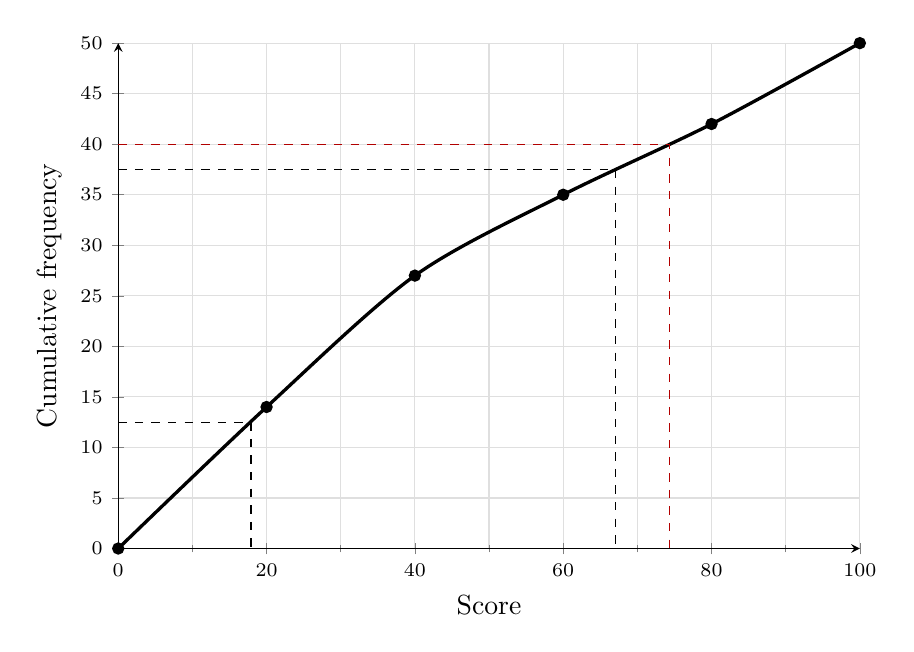
\begin{tikzpicture}
\begin{axis}[
  width=11cm, height=8cm,
  xmin=0, xmax=100, ymin=0, ymax=50,
  xtick={0,20,40,60,80,100}, ytick={0,5,10,15,20,25,30,35,40,45,50},
  minor x tick num=1,
  xlabel={Score}, ylabel={Cumulative frequency},
  grid=both, grid style={gray!25},
  tick label style={font=\scriptsize},
  axis lines=left]
  \addplot[very thick, smooth, mark=*, mark size=1.6pt]
    coordinates {(0,0) (20,14) (40,27) (60,35) (80,42) (100,50)};
  \draw[dashed] (axis cs:0,12.5) -- (axis cs:17.9,12.5) -- (axis cs:17.9,0);
  \draw[dashed] (axis cs:0,37.5) -- (axis cs:67.1,37.5) -- (axis cs:67.1,0);
  \draw[dashed, red!70!black] (axis cs:0,40) -- (axis cs:74.3,40) -- (axis cs:74.3,0);
\end{axis}
\end{tikzpicture}
\end{center}

\textbf{(a)} There are $50$ adults.
\[ \text{lower quartile at } \frac{50}{4} = 12.5 \qquad \text{upper quartile at } \frac{3 \times 50}{4} = 37.5 \]
Read across from $12.5$ and from $37.5$ to the curve, then down to the score axis.
\[ \mathrm{LQ} \approx 18 \qquad \mathrm{UQ} \approx 67 \]
\[ \mathrm{IQR} \approx 67 - 18 = 49 \]
Any pair of readings taken correctly from the curve, then subtracted, is accepted.

\textbf{(b)} The prize-winners are the top $20\%$ of the $50$ adults.
\[ 20\% \text{ of } 50 = 10 \text{ adults} \]
So $50 - 10 = 40$ adults score less than the minimum. Read across from $40$ on the cumulative frequency axis and down to the score axis.
\[ \text{minimum score} \approx 75 \]

\textbf{(c)} Read the cumulative frequency at the end of each interval, then subtract consecutive readings to recover each frequency.
\[ 20 \to 14 \qquad 40 \to 27 \qquad 60 \to 35 \qquad 80 \to 42 \qquad 100 \to 50 \]
\[ 0 < s \leqslant 20: \quad 14 - 0 = 14 \]
\[ 20 < s \leqslant 40: \quad 27 - 14 = 13 \]
\[ 40 < s \leqslant 60: \quad 35 - 27 = 8 \]
\[ 60 < s \leqslant 80: \quad 42 - 35 = 7 \]
The last frequency, $8$, is already given, and the five add to $50$ as they must.
\end{ansbox}

%========================= Q19 =========================
\examq{4024/11/O/N/24}{19}{Proportion}{2}

\begin{mstab}{q9color}
19 & $\dfrac{1}{16}$ oe nfww \newline B1 for $k = 8$ if $y = \dfrac{k}{x}$ used \newline or M1 for $2 \times \sqrt{16} = 32 \times \sqrt{y}$ oe \newline or M1FT for $\sqrt{y} = \dfrac{\text{their } k}{32}$ & 2 \\ \hline
\end{mstab}

\begin{ansbox}{q9color}
Inverse proportion to the square root of $y$ means
\[ x = \frac{k}{\sqrt{y}} \]
Substitute the given pair $x = 2$, $y = 16$ to find $k$.
\[ 2 = \frac{k}{\sqrt{16}} = \frac{k}{4} \]
\[ k = 8 \]
So $x\sqrt{y} = 8$. Now put $x = 32$.
\[ 32 = \frac{8}{\sqrt{y}} \]
\[ \sqrt{y} = \frac{8}{32} = \frac{1}{4} \]
Square both sides.
\[ y = \frac{1}{16} \]
\end{ansbox}

%========================= Q20 =========================
\examq{4024/11/O/N/24}{20}{Algebraic Roots \& Indices}{2}

\begin{mstab}{q10color}
20 & $[a =]\ 8$ \newline $[n =]\ 15$ \newline B1 for each & 2 \\ \hline
\end{mstab}

\begin{ansbox}{q10color}
Deal with the number and the power of $x$ separately in
\[ \left(4x^{10}\right)^{\frac{3}{2}} = ax^{n} \]
For the number, a power of $\tfrac{3}{2}$ means square root first, then cube.
\[ 4^{\frac{3}{2}} = \left(\sqrt{4}\right)^3 = 2^3 = 8 \]
For the $x$ part, use $(x^{m})^{p} = x^{mp}$.
\[ \left(x^{10}\right)^{\frac{3}{2}} = x^{10 \times \frac{3}{2}} = x^{15} \]
Putting these together:
\[ \left(4x^{10}\right)^{\frac{3}{2}} = 8x^{15} \]
\[ a = 8 \qquad n = 15 \]
\end{ansbox}

%========================= Q21 =========================
\examq{4024/11/O/N/24}{21}{Real-Life Graphs}{2}

\begin{mstab}{q1color}
21 & 400 \newline M1 for attempt to find a relevant area under the graph soi by e.g. $\left(\dfrac{60 + 20}{2}\right) \times 10$, $\dfrac{10 \times 10}{2}$, $(30 - 10) \times 10$, $\dfrac{(60 - 30) \times 10}{2}$ oe & 2 \\ \hline
\end{mstab}

\begin{ansbox}{q1color}
\begin{center}
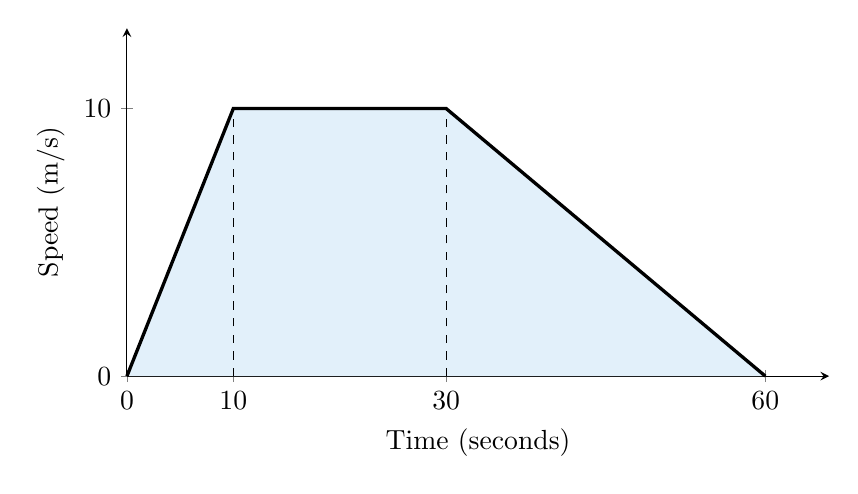
\begin{tikzpicture}
\begin{axis}[
  width=10.5cm, height=6cm,
  axis lines=left,
  xmin=0, xmax=66, ymin=0, ymax=13,
  xtick={0,10,30,60}, ytick={0,10},
  xlabel={Time (seconds)}, ylabel={Speed (m/s)},
  clip=false]
  \draw[fill=q1color!70, draw=none]
    (axis cs:0,0) -- (axis cs:10,10) -- (axis cs:30,10) -- (axis cs:60,0) -- cycle;
  \addplot[very thick] coordinates {(0,0) (10,10) (30,10) (60,0)};
  \draw[dashed] (axis cs:10,0) -- (axis cs:10,10);
  \draw[dashed] (axis cs:30,0) -- (axis cs:30,10);
\end{axis}
\end{tikzpicture}
\end{center}

Distance travelled is the area under a speed--time graph. The shape is a trapezium, so it can be taken either in three pieces or in one.

\textbf{In three pieces:}
\[ \text{triangle } (0 \text{ to } 10) = \frac{1}{2} \times 10 \times 10 = 50 \]
\[ \text{rectangle } (10 \text{ to } 30) = (30 - 10) \times 10 = 200 \]
\[ \text{triangle } (30 \text{ to } 60) = \frac{1}{2} \times (60 - 30) \times 10 = 150 \]
\[ \text{total} = 50 + 200 + 150 = 400 \]

\textbf{As one trapezium}, with parallel sides $60$ and $30 - 10 = 20$, and height $10$:
\[ \left(\frac{60 + 20}{2}\right) \times 10 = 40 \times 10 = 400 \]
The total distance travelled is $400\ \mathrm{m}$.
\end{ansbox}

%========================= Q22 =========================
\examq{4024/11/O/N/24}{22}{Quadratic Equations \textperiodcentered\ Functions}{4}

\begin{mstab}{q2color}
22(a) & 8 & 1 \\ \hline
22(b) & 1 or $-1$ nfww \newline B2 for $12x^2 - 12 = 0$ or $12x^2 = 12$ or better \newline or M1 for $3(2x)^2 + 5 = 17$ oe soi & 3 \\ \hline
\end{mstab}

\begin{ansbox}{q2color}
Throughout, $\mathrm{f}(x) = 3x^2 + 5$.

\textbf{(a)} Substitute $x = -1$, squaring before multiplying.
\[ \mathrm{f}(-1) = 3(-1)^2 + 5 = 3(1) + 5 = 8 \]

\textbf{(b)} Replace every $x$ in the rule by $2x$.
\[ \mathrm{f}(2x) = 3(2x)^2 + 5 \]
Note that $(2x)^2 = 4x^2$, not $2x^2$.
\[ 3 \times 4x^2 + 5 = 17 \]
\[ 12x^2 + 5 = 17 \]
\[ 12x^2 = 12 \]
\[ x^2 = 1 \]
A square root has two values.
\[ x = 1 \qquad \text{or} \qquad x = -1 \]
\end{ansbox}

%========================= Q23 =========================
\examq{4024/11/O/N/24}{23}{Rounding, Estimation \& Bounds}{2}

\begin{mstab}{q3color}
23(a) & 32.5 & 1 \\ \hline
23(b) & 18 & 1 \\ \hline
\end{mstab}

\begin{ansbox}{q3color}
\textbf{(a)} Correct to the nearest centimetre means the true length is within $0.5\,\mathrm{cm}$ either side.
\[ \text{upper bound} = 32 + 0.5 = 32.5\ \mathrm{cm} \]

\textbf{(b)} A difference is largest when the number being subtracted is as \emph{small} as possible. So take the upper bound of the length and the \textbf{lower} bound of the width.
\[ \text{length upper bound} = 32.5 \qquad \text{width lower bound} = 15 - 0.5 = 14.5 \]
\[ 32.5 - 14.5 = 18 \]
The upper bound for the difference is $18\ \mathrm{cm}$.
\end{ansbox}

%========================= Q24 =========================
\examq{4024/11/O/N/24}{24}{Algebraic Fractions}{3}

\begin{mstab}{q4color}
24 & $\dfrac{2x - 1}{2x}$ or $1 - \dfrac{1}{2x}$ final answer nfww \newline B1 for $(2x - 1)(x + 3)$ seen \newline B1 for $2x(x + 3)$ seen & 3 \\ \hline
\end{mstab}

\begin{ansbox}{q4color}
Factorise the numerator and the denominator separately.

Numerator: $2x^2 + 5x - 3$. Two numbers multiplying to $2 \times (-3) = -6$ and adding to $5$ are $6$ and $-1$.
\[ 2x^2 + 6x - x - 3 = 2x(x + 3) - 1(x + 3) = (2x - 1)(x + 3) \]
Denominator: take out the common factor $2x$.
\[ 2x^2 + 6x = 2x(x + 3) \]
Now cancel the common factor $(x + 3)$.
\[ \frac{2x^2 + 5x - 3}{2x^2 + 6x} = \frac{(2x - 1)(x + 3)}{2x(x + 3)} = \frac{2x - 1}{2x} \]
This may also be written as $1 - \dfrac{1}{2x}$.
\end{ansbox}

%========================= Q25 =========================
\examq{4024/11/O/N/24}{25}{3D Pythagoras \& Trigonometry}{3}

\begin{mstab}{q5color}
25 & 3 nfww \newline M2 for $\sqrt{7^2 - 6^2 - 2^2}$ oe soi \newline or M1 for any correct 2D Pythagoras pair e.g. $2^2 + 6^2$, $7^2 - 6^2$ or $7^2 - 2^2$ oe or better seen & 3 \\ \hline
\end{mstab}

\begin{ansbox}{q5color}
$EC$ runs from one corner of the cuboid to the opposite corner, so it is a space diagonal. For a cuboid with edges $p$, $q$, $r$ the space diagonal $d$ satisfies
\[ d^2 = p^2 + q^2 + r^2 \]
Here the three edge lengths meeting at that diagonal are $EH = 6$, $HG = 2$ and the unknown $CG$, with $EC = 7$.
\[ 7^2 = 6^2 + 2^2 + CG^2 \]
\[ 49 = 36 + 4 + CG^2 \]
\[ CG^2 = 49 - 40 = 9 \]
\[ CG = 3 \]
$CG = 3\ \mathrm{cm}$.

The same result in two steps: the diagonal of the face $EHGF$ is $EG = \sqrt{6^2 + 2^2} = \sqrt{40}$, and then triangle $ECG$ is right-angled at $G$, so
\[ CG = \sqrt{7^2 - 40} = \sqrt{9} = 3 \]
\end{ansbox}

%========================= Q26 =========================
\examq{4024/11/O/N/24}{26}{Algebraic Fractions}{4}

\begin{mstab}{q6color}
26 & 2 nfww \newline B3 for $2x^2 - x - 3x + 3 = 2x^2 - 2x - x + 1$ or better \newline or M2 for an equation with fractions eliminated or for correct use of common denominator in an equation, accept LHS as two fractions \newline or M1 for $x(2x - 1) - 3(x - 1)$ or common denominator $(2x - 1)(x - 1)$ soi & 4 \\ \hline
\end{mstab}

\begin{ansbox}{q6color}
The equation is
\[ \frac{x}{x - 1} - \frac{3}{2x - 1} = 1 \]
Multiply every term by the common denominator $(x - 1)(2x - 1)$.
\[ x(2x - 1) - 3(x - 1) = (x - 1)(2x - 1) \]
Expand all of the brackets.
\[ 2x^2 - x - 3x + 3 = 2x^2 - 2x - x + 1 \]
\[ 2x^2 - 4x + 3 = 2x^2 - 3x + 1 \]
The $2x^2$ terms cancel.
\[ -4x + 3 = -3x + 1 \]
\[ 3 - 1 = -3x + 4x \]
\[ x = 2 \]

Check: $\dfrac{2}{2 - 1} - \dfrac{3}{4 - 1} = 2 - 1 = 1$ \checkmark
\end{ansbox}

\end{document}